\title{JACK (JACK Audio Connection Kit) and related tools}

\maketitle
\tableofcontents

\chapter{The server}

\section{What is \href{http://jackaudio.org/}{JACK}?}
%{{{ 
\begin{itemize}
\item JACK is a sound system (audio server) for POSIX operating
  systems (such as Linux, FreeBSD, MacOS X and Windows XP).
\item It is a software layer between the kernel (ALSA) and the
  applications that requires to access to the sound hardware.
\item Licensed under \href{https://www.gnu.org/licenses/lgpl.html}{LGPL}.
\end{itemize}

%}}}

\section{Functions}
%{{{ 

\begin{itemize}
\item Controllable latency (suitable real-time audio applications).
\item Allow to define the connections (audio flows) between JACK-client
  applications (like in a real mixer desk).
\item \href{http://www.linuxjournal.com/node/1004080}{Transport
    control synchronization.} JACK can send timming events (using the
  JACK transport control system) to the rest of clients in order to
  synchronize them.
\item \href{http://en.wikipedia.org/wiki/MIDI}{MIDI} capabilities.
\end{itemize}

%}}}

\section{Installation}
%{{{

\begin{enumerate}
% \begin{comment}
% \item Add yourself to the \texttt{audio} group. Otherwise, only the
%   \texttt{root} can use JACK.
  
% \begin{verbatim}
% sudo adduser $USER audio
% \end{verbatim}

% \item Change to the \texttt{audio} group:
  
% \begin{verbatim}
% newgrp audio
% \end{verbatim}
% \end{comment}  

\item Install the program \texttt{qjackctl}. This a graphical
  front-end for controlling the audio server \texttt{jackd2}. During
  the installation of \texttt{jackd} you must decide to enable the
  realtime process priority (necesarry for real-time processing in
  slow systems). The priority is defined in the file:

\begin{verbatim}
$ cat /etc/security/limits.d/audio.conf 
# Provided by the jackd package.
#
# Changes to this file will be preserved.
#
# If you want to enable/disable realtime permissions, run
#
#    dpkg-reconfigure -p high jackd

@audio   -  rtprio     95
@audio   -  memlock    unlimited
#@audio   -  nice      -19
\end{verbatim}

\end{enumerate}
% \begin{comment}
%   Vamos a instalar JACK a
%   partir de otro programa (muy b'asico) que lo necesita. Dicho
%   programa es Meterbridge y se trata de un v'umetro (un dispositivo
%   que mide el nivel de volumen en tiempo real de la se\~nal de audio):
% \begin{verbatim}
% sudo apt-get install meterbridge

% # Instala entre otros, los paquetes "jackd" (el demonio para jack),
% # "qjackctl" (el controlador del demonio llamado "JACK Control") y
% # "meterbridge (un vol'umetro). Estas dos 'ultimas aplicaciones son
% # gr'aficas y aparecen en el men'u desplegable.

% # A la pregunta de que si se desea ejecutar "jackd" en tiempo real,
% # indicar s'i (aunque deber'ia tenerse en cuenta que sin un kernel RT
% # (Real-Time) "jackd" podr'ia generar "XRuns" (p'erdida de datos de
% # audio)".

% # El paquete "jackd" ha debido generar el fichero:
% #
% # /etc/security/limits.d/audio.conf
% #
% # Que indica los privilegios necesarios para usar el driver de
% # audio Jack. Si lo visualizamos podemos ver dos cosas:
% # 1. Que se manipula a trav'es de "dpkg-reconfigure -p high jackd".
% # 2. Que para poder obtener estos privilegios, el usuario deber'ia
% # pertenecer al grupo "audio".

% # Para pertenercer al grupo "audio" primero tenemos que verificar si
% # existe o no:
% X=`grep audio /etc/group` # Ojo con estas comillas.
% # Son las que est'an a la derecha de la tecla "P".
% echo $X

% # Si el anterior comando devuelve algo semejante a:
% # "audio:x:29:pulse" es que el grupo est'a creado. Si no fuera as'i,
% # habr'ia que crearlo con el comando "groupadd".

% # Y una vez que el grupo "audio" existe, nos a~nadimos al mismo:
% sudo cp /etc/group /etc/group.old
% rm -f /tmp/1
% sed -e "s/$X/$X,$USER/g" /etc/group.old > /tmp/1
% sudo mv /tmp/1 /etc/group

% # También hay que añadir tu nombre de usuario al fichero /etc/gshadow

% # Ahora cerramos la sesi'on y volvemos a entrar.
% \end{verbatim}
% \end{comment}

%}}}

\section{JACK graphical front-end: \href{http://qjackctl.sourceforge.net/}{qjackctl}}
%{{{

\begin{itemize}
\item Provides a simple GUI dialog for setting several JACK daemon
  parameters, which are properly saved between sessions, and a way
  control of the status of the audio server daemon. Run it with:
\begin{verbatim}
$ qjackctl &
\end{verbatim}
\begin{center}
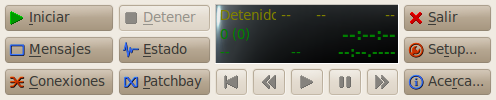
\includegraphics{qjackctl}
\end{center}
\item Control actions:
\begin{enumerate}
\item \texttt{Start:} the server.
\item \texttt{Stop:} the server.
\item \texttt{Quit:} kill the server.
\item \texttt{Messages:} from the server.
\item \texttt{Session:} show/hide the session manager window.
\item \texttt{Setup:} the server. 
\item \texttt{Connect:} the audio
  applications. \href{http://www.rncbc.org/drupal/node/76}{Notice
    that} all connections made in the Connections interface are kept
  as long you don't power-cycle the JACK server (jackd). That is, all
  connections will be lost when the JACK server or any of the client
  application programs are closed or terminated.
\item \texttt{Patchbay:} will keep all declared connections
  automatically, as long as QjackCtl is kept alive. Moreover, you can
  declare typical connection configuration that are carried out when
  the related clients are executed.
\item Play: start transport timming events.
\item Pause: stop transport timming events.
\item Forward: transport timming events.
\item Backward: transport timming event.
\item Rewind: transport timming event.
\end{enumerate}
\end{itemize}

%}}}

\subsection{Server configuration}
%{{{

\begin{itemize}
\item Select the Setup form from the \texttt{qjackctl}
  application. Clicking in the "Settings" tab, you will obtain
  something like:
  \begin{center}
    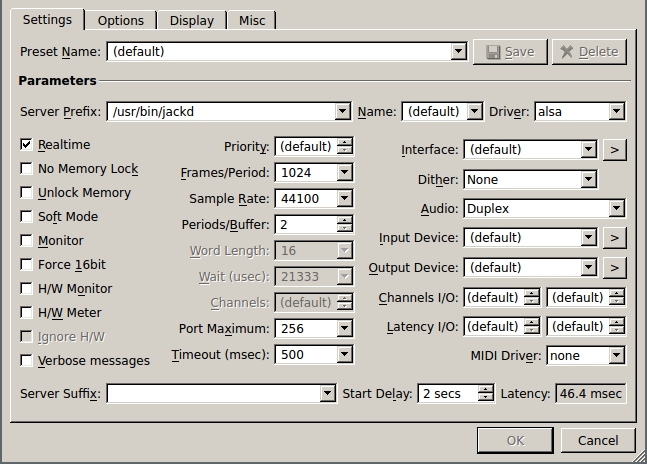
\includegraphics{jack-setup}
  \end{center}
\item Among others, the Setup window allows you to configure
  \href{http://en.flossmanuals.net/ardour/ch015_starting-jack-on-ubuntu/}{important
    settings}:
  \begin{enumerate}
  \item \textbf{Driver:} the physical audio driver. On Linux, the
    default option is ALSA.
  \item \textbf{Realtime:} although this option is selected as the
    default, it requires a Real-time capable system to use. Unless you
    have configured your operating system for Real-time, uncheck this
    option.
  \item \textbf{Interface:} select the physical audio device that you
    would like the Jack server to communicate with (for example, a
    FireWire or USB interface or the built-in audio of your
    computer). Currently, JACK can only communicate with one hardware
    audio device at a time.
  \item \textbf{Frames/Period:} choose your desired audio buffer size
    (in samples=frames). This paremeter controls the Latency.
  \item \textbf{Sample Rate:} choose your desired sample rate for the
    Jack server and the rest of clients.
\end{enumerate}

\item Once you have chosen your settings, click on OK to exit the Setup
window. Note that however the new settings will be saved, you will
have to restart the JACK Server for the changes to take effect.

\end{itemize}

%}}}

\section{Minimizing the number of XRUNs}

\begin{itemize}

\item When we play live music with a computer, it is very
  important a low latency. This aspect can be controlled in the Setup
  section of JACK modifying the buffer size.

\item However, Linux is a multi-task OS and JACK competes for the same
  resources that other applications. Therefore, when Jack does not
  gets enough CPU a XRUN is provoked and the playback stutters.

\item In order to minimize the number of XRUNs we should realise that:

  \begin{enumerate}

  \item Run only the critical applications.

  \item The JACK server is running with the highest
    priority\footnote{The priority of a process can change between -20
      and 20. The lower this value, higher priority.}. The current
    priority can be determined by:

%\begin{verbatim}
%X=`ps -C jackd -o pid=`; ps -o nice -p $X
%\end{verbatim}
\begin{lstlisting}
X=`ps -C jackd -o pid=`; ps -o nice -p $X
\end{lstlisting}

    And incremented with:

\begin{verbatim}
X=`ps -C jackd -o pid=`; sudo renice -20 -p $X
# Notice that renice only runs with administrator privileges!
\end{verbatim}

  \item Configure, compile and boot a
    \href{https://rt.wiki.kernel.org/index.php/Main_Page}{real-time
      kernel}.

  \item Improve your sound hardware.

  \item Improve your computer hardware.

  \end{enumerate}
\end{itemize}

\chapter{Living with PulseAudio}

\section{What is \href{http://www.freedesktop.org/wiki/Software/PulseAudio/About/}{Pulseaudio?}}

\begin{itemize}
\item Pulseaudio is a sound system (audio server) for POSIX operating
  systems (such as GNU/Linux, Solaris, FreeBSD, NetBSD, MacOS X,
  Windows 2000 and Windows XP).

\item It is a software layer between the kernel (ALSA) and the
  applications that requires to access to the sound hardware.

\item \href{https://rudd-o.com/linux-and-free-software/how-pulseaudio-works}{Architecture}:
\begin{center}
  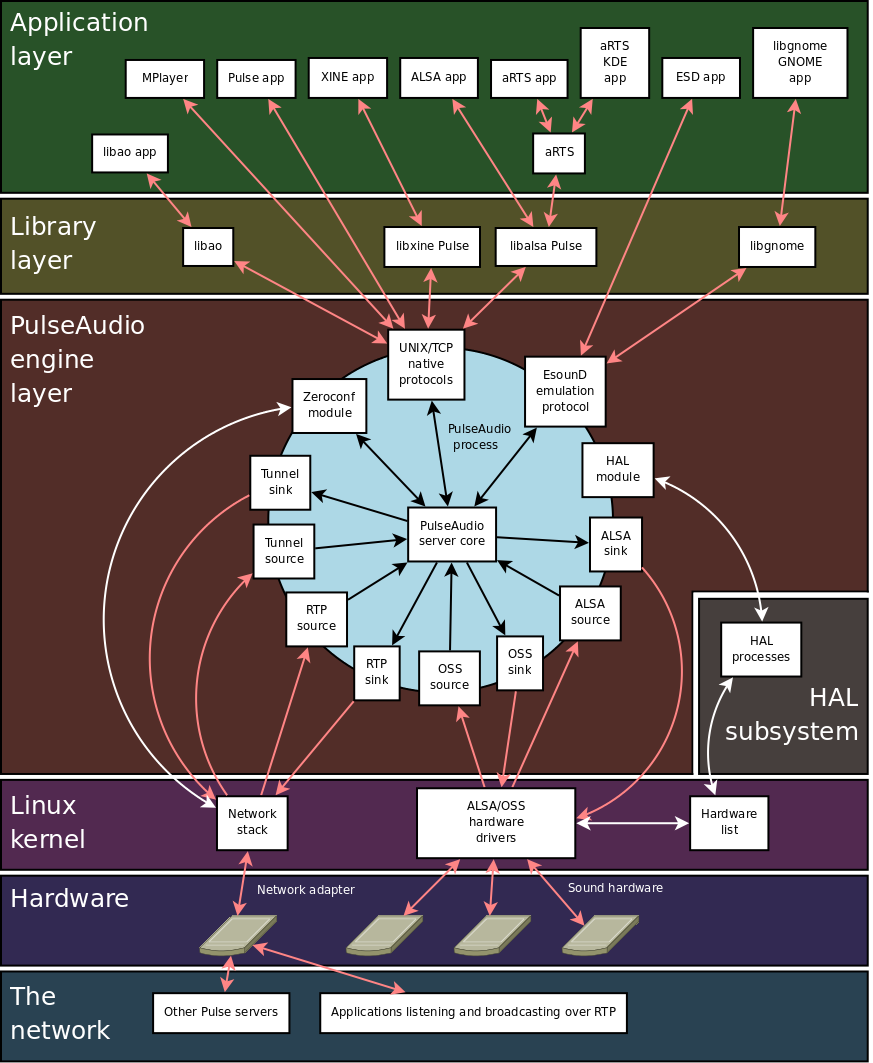
\includegraphics{PulseAudio_diagram}
\end{center}

\item Licensed under LGPL 2.1+.

\item Currently, PulseAudio (PA) is used in most friendly Linux
  distributions to multiplex the sound hardware between the
  applications that use it.

\item The server and clients does not need to run in the same
  host. This means that one application that run in a remote host can
  play sound in the local host of the user (that runs the server).

\end{itemize}

\section{Functions}
\begin{enumerate}
\item Software mixing of multiple audio streams, bypassing any
  restrictions the hardware has.
\item Network transparency, allowing an application to play back or
  record audio on a different machine than the one it is running on.
\item Sound API abstraction, alleviating the need for multiple
  backends in applications to handle the wide diversity of sound
  systems out there.
\item Generic hardware abstraction, giving the possibility of doing
  things like individual volumes per application.
\end{enumerate}

\section{\href{https://wiki.archlinux.org/index.php/PulseAudio}{Daemon control}}
\begin{itemize}

\item In the unlikely case that PulseAudio is not automatically
  started upon entering X, it can can be started with:
\begin{verbatim}
ps aux | grep pulse
...
vruiz     2201  0.0  0.2 484192  5728 ?        Sl   Sep17  32:18 /usr/bin/pulseaudio --start --log-target=syslog
vruiz     2204  0.0  0.0  98392   508 ?        S    Sep17   0:00 /usr/lib/pulseaudio/pulse/gconf-helper
vruiz    20709  0.0  0.0  11748   888 pts/13   S+   17:13   0:00 grep pulse
...

pulseaudio --start   # On the whole system
start-pulseaudio-x11 # In a X session (usually inside ~/.xinitrc)
\end{verbatim}
and stopped with:
\begin{verbatim}
pulseaudio --kill
\end{verbatim}

\item A more accurate control can be obtained with
  \texttt{pactl}. More info at \texttt{man pactl}.

\end{itemize}

\section{Pulseaudio and ALSA tools}
\begin{itemize}
\item By default, in most OSs, ALSA tools (such as \texttt{arecord})
  has been configured to access to the sound hardware thought
  Pulseaudio.
\end{itemize}

\section{Bypassing PA server (and JACK)}
\begin{verbatim}
pasuspender mplayer -ao alsa * &
\end{verbatim}

\section{Sound system usage}
\begin{verbatim}
$ fuser -v /dev/snd/*
                     USER        PID ACCESS COMMAND
/dev/snd/controlC0:  vruiz      2201 F.... pulseaudio
                     vruiz      3810 F.... alsamixer
/dev/snd/pcmC0D0p:   vruiz      2201 F...m pulseaudio
\end{verbatim}

\section{Configuration}
PA is configured by modifiying the files:
\begin{verbatim}
/etc/pulse/daemon.conf
/etc/pulse/default.pa
\end{verbatim}

\section{Volume control}
\begin{verbatim}
$ pavucontrol &
\end{verbatim}

\section{Module \texttt{pulseaudio-module-jack}}
\begin{verbatim}
# Install the PulseAudio's module for Jack
sudo apt-get install pulseaudio-module-jack

# Go to:
cd /etc/pulse/

# Make a backup of the file:
sudo cp default.pa default.pa.old

# Edit it:
sudo gedit default.pa

# Add:
#
# load-module module-jack-source
# load-module module-jack-sink
#
# after "load-module module-pipe-sink".
#
# Remember to remove the '#' of these lines!!

# Kill and reload JACK.
pulseaudio --kill
\end{verbatim}
\begin{center}
  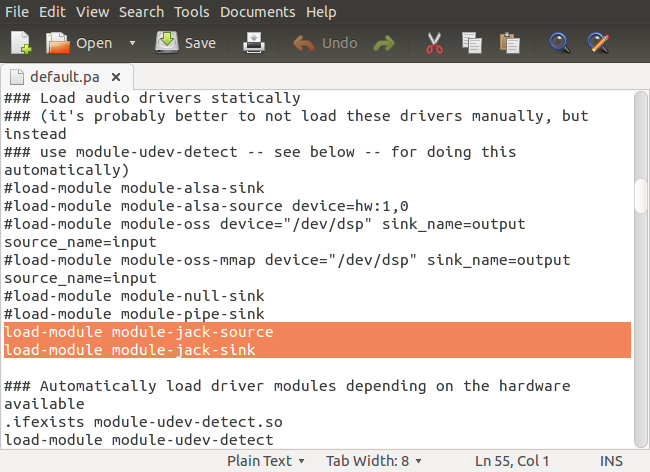
\includegraphics{gedit}
  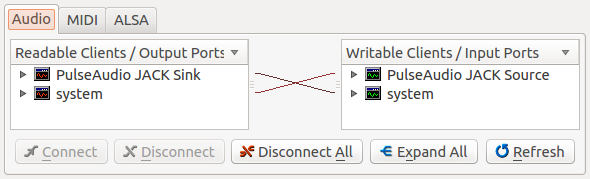
\includegraphics{pulse-connections}
\end{center}

\chapter{Media players}

\section{Media player: \href{http://www.mplayerhq.hu/}{MPlayer}}
%{{{

\begin{verbatim}
$ mplayer -ao jack * &
\end{verbatim}
\begin{center}
  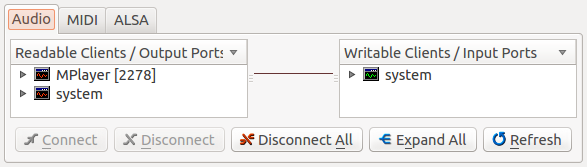
\includegraphics{mplayer-connections}
  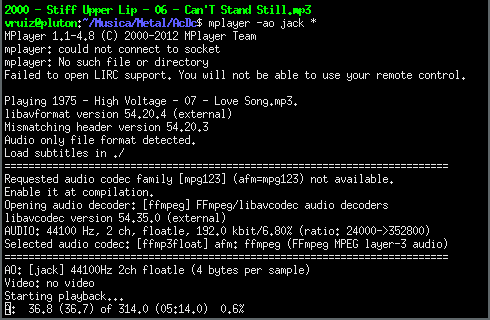
\includegraphics{mplayer}
  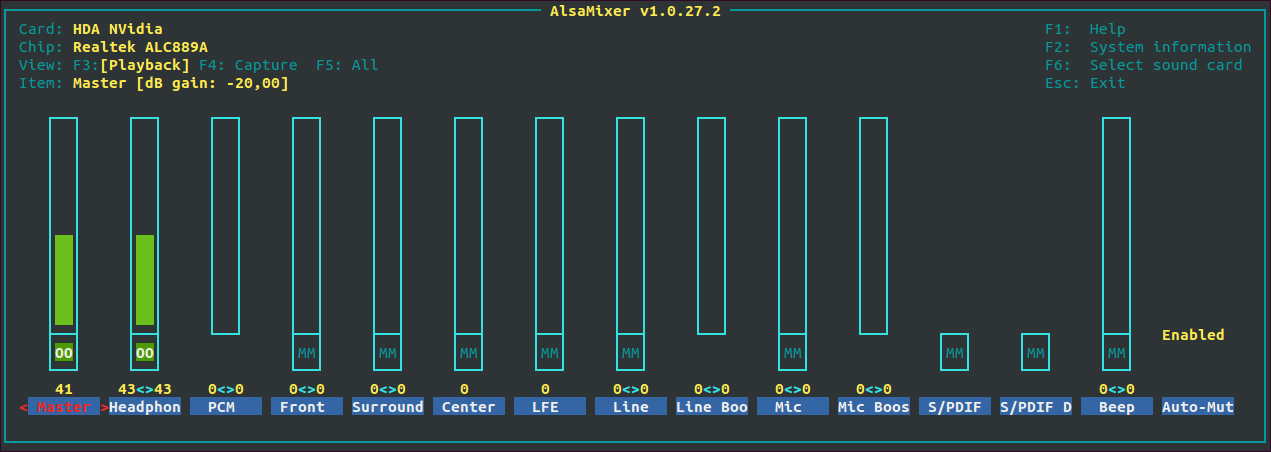
\includegraphics{mplayer-alsamixer}
\end{center}

%}}}

% \begin{comment}

% \section{Audio player: \href{http://aqualung.factorial.hu/}{Aqualung}}
% %{{{

% \begin{verbatim}
% $ aqualung &
% \end{verbatim}
% \begin{center}
%   \includegraphics{Aqualung-connections} %
%   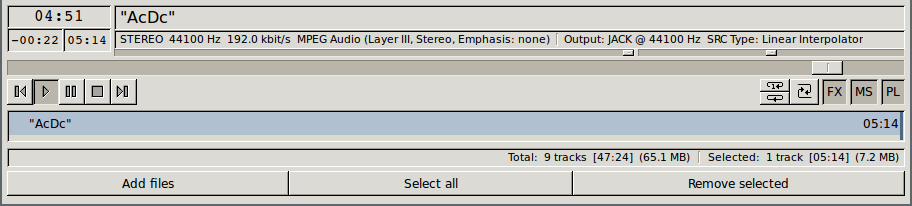
\includegraphics{Aqualung}
% \end{center}

% %}}}

% \end{comment}

\chapter{Meters}

\section{A VU (Volume Unit) meter: \href{http://plugin.org.uk/meterbridge/}{meterbridge}}
%{{{

\begin{enumerate}
\item Run:
\begin{verbatim}
$ meterbridge -t vu alsa_pcm:capture_1 alsa_pcm:capture_2 &  # Or ...
$ meterbridge -t ppm alsa_pcm:capture_1 alsa_pcm:capture_2 & # Or ...
$ meterbridge -t dpm alsa_pcm:capture_1 alsa_pcm:capture_2 & # Or ...
$ meterbridge -t jf alsa_pcm:capture_1 alsa_pcm:capture_2 &  # Or ...
$ meterbridge -t sco alsa_pcm:capture_1 alsa_pcm:capture_2 & # Although this is preferable
\end{verbatim}
\begin{center}
  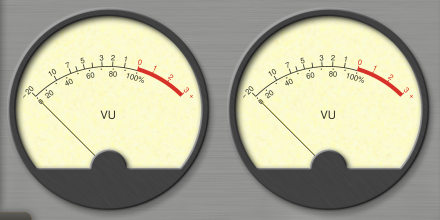
\includegraphics{meterbridge}
\end{center}
\item Connect (route) it:
\begin{center}
  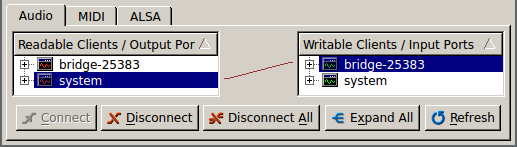
\includegraphics{qjackctl-meterbridge}
\end{center}

\item But, I don't listen myself! Of course, you have to route the
  \texttt{system} readable client in the Connections/Audio window
  towards the \texttt{system} writable client in order to provide this
  functionality. But be careful with the output volume of the speakers
  (Master and PCM) and the microphone gain (Mic and Mic Boost) mixer
  controls, specially is you are done this in a laptop, because the
  microphone can be feedbacked by the speakers, producing an annoying
  sound coupling. See below:

  \begin{center}
    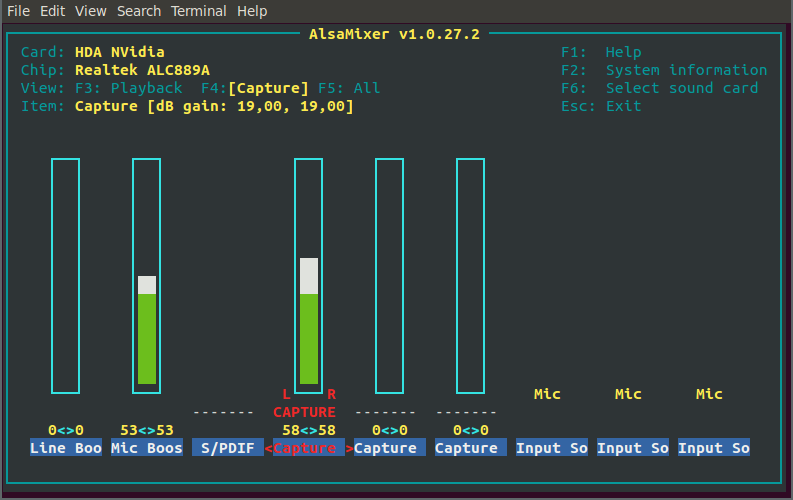
\includegraphics{alsamixer-capture}
    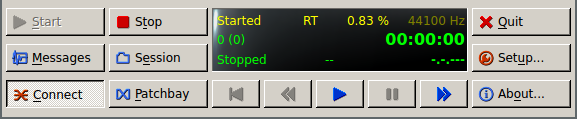
\includegraphics{JACK-started}
    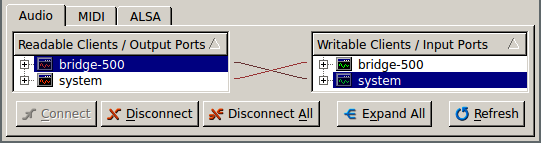
\includegraphics{meterbridge-connections}
    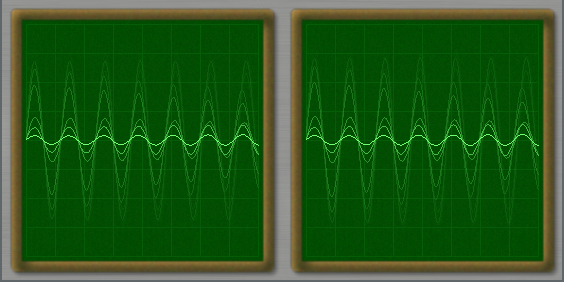
\includegraphics{meterbridge-sco}
  \end{center}
  
\end{enumerate}

%}}}

% \begin{comment}

% \section{\href{http://www.kokkinizita.net/linuxaudio/}{Jaaa (JACK and Alsa Audio Analyser)}}
% %{{{

% \begin{itemize}
% \item Run as (while the JACK server is running):
% \begin{verbatim}
% $ jaaa -J &
% \end{verbatim}
%   \begin{center}
%   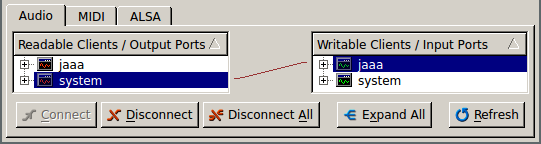
\includegraphics{jaaa-connections}
%   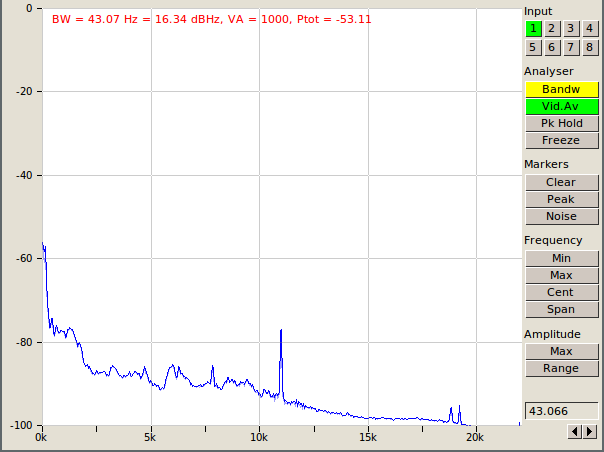
\includegraphics{jaaa}
%   \end{center}
% \item Notice that is a mono analyzer.
% \end{itemize}

% %}}}

% \end{comment}

\section{\href{http://www.kokkinizita.net/linuxaudio/}{Japa (JACK Perceptual Analyzer)}}
%{{{

\begin{itemize}
\item Run as (while the JACK server is running):
\begin{verbatim}
$ japa -J &
\end{verbatim}
  \begin{center}
    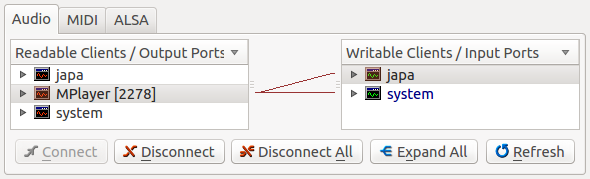
\includegraphics{japa-connections}
    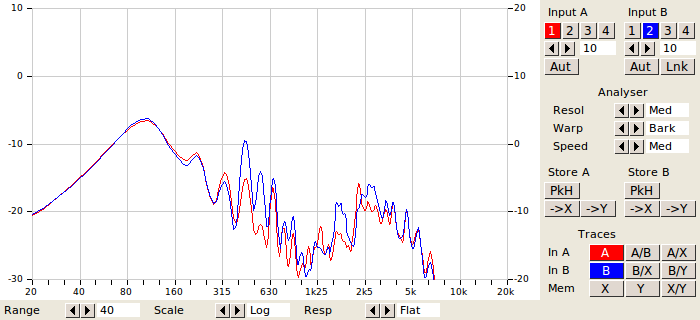
\includegraphics{japa}
  \end{center}
\end{itemize}

%}}}

\chapter{Effects}

\section{\href{http://jamin.sourceforge.net}{JAMin (JACK Audio Mastering interface)}}
%{{{

\begin{verbatim}
$ jamin &
\end{verbatim}
\begin{center}
  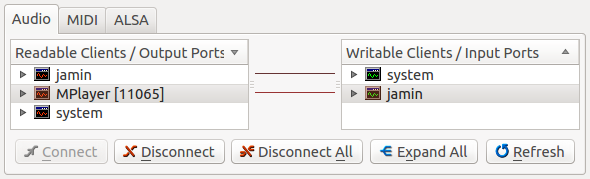
\includegraphics{jamin-connections}
  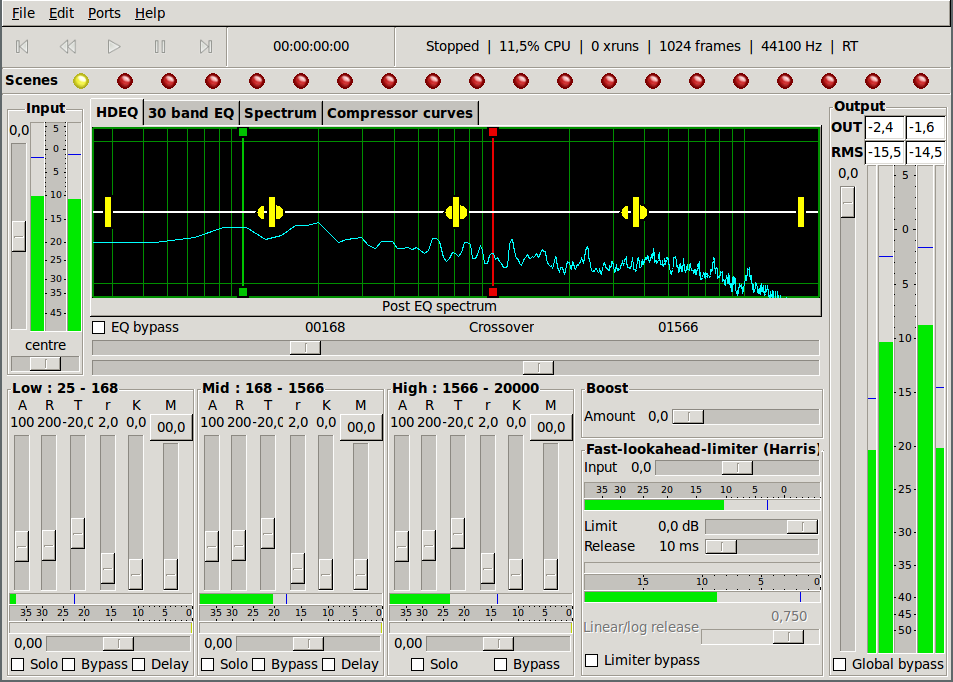
\includegraphics{jamin}
\end{center}

%}}}

% \begin{comment}

% \section{\href{http://ardour.org}{Ardour}}
% %{{{

% \begin{verbatim}
% $ ardour2 &
% \end{verbatim}
% \begin{center}
%   \includegraphics{ardour-connections}
%   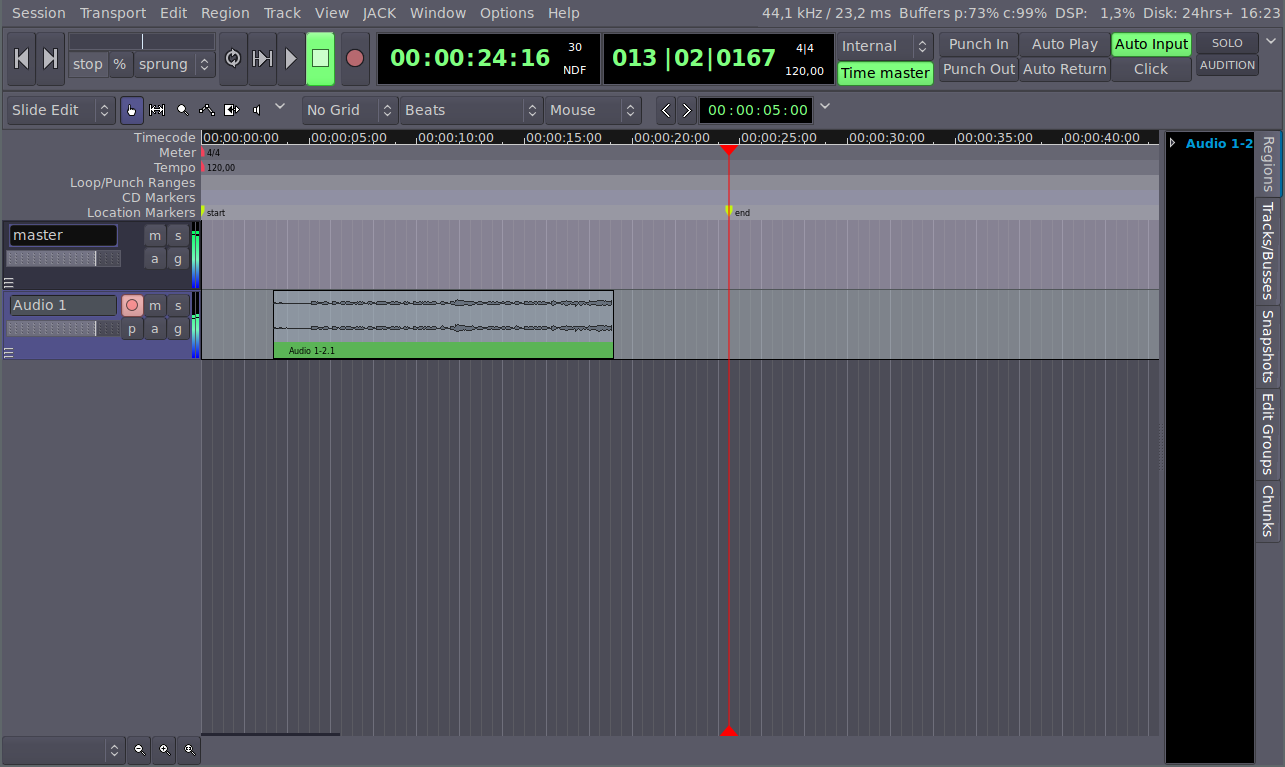
\includegraphics{ardour}
% \end{center}

% %}}}

% \end{comment}

\section{\href{http://jack-rack.sourceforge.net}{JACK Rack}}
\begin{verbatim}
$ jack-rack &
\end{verbatim}
\begin{center}
  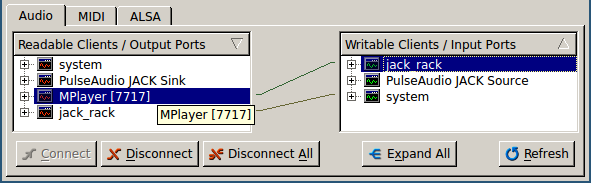
\includegraphics{jack-rack-connections}
  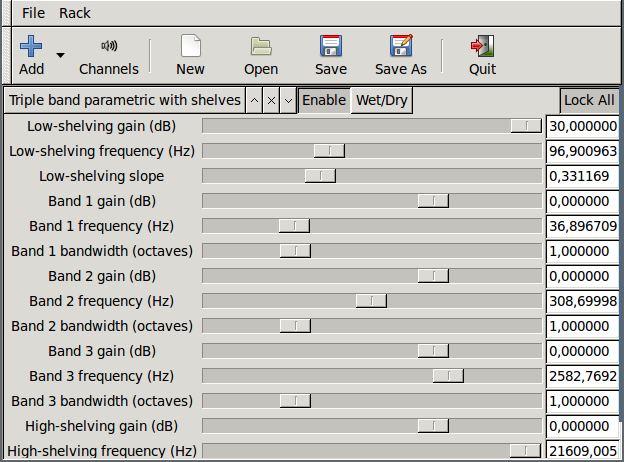
\includegraphics{jack-rack}
\end{center}

\section{\href{http://rakarrack.sourceforge.net}{Rakarrack}}
\begin{verbatim}
$ rakarrack &
\end{verbatim}
\begin{center}
  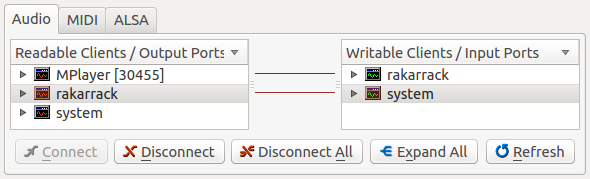
\includegraphics{rakarrack-connections}  
  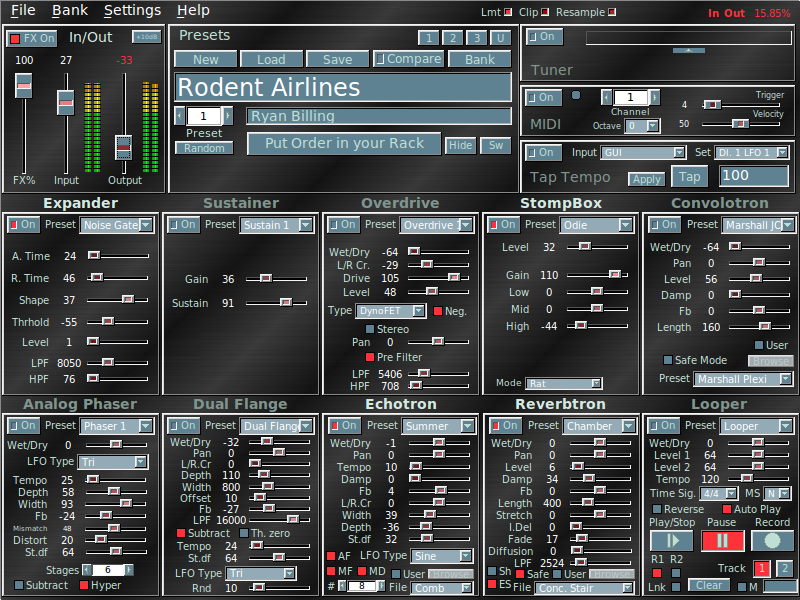
\includegraphics{rakarrack}
\end{center}

\section{\href{http://freqtweak.sourceforge.net}{Freqtweak}}
\begin{verbatim}
$ freqtweak &
\end{verbatim}
\begin{center}
  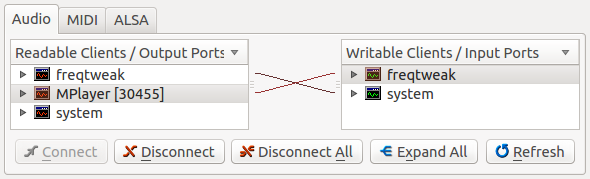
\includegraphics{freqtweak-connections}  
  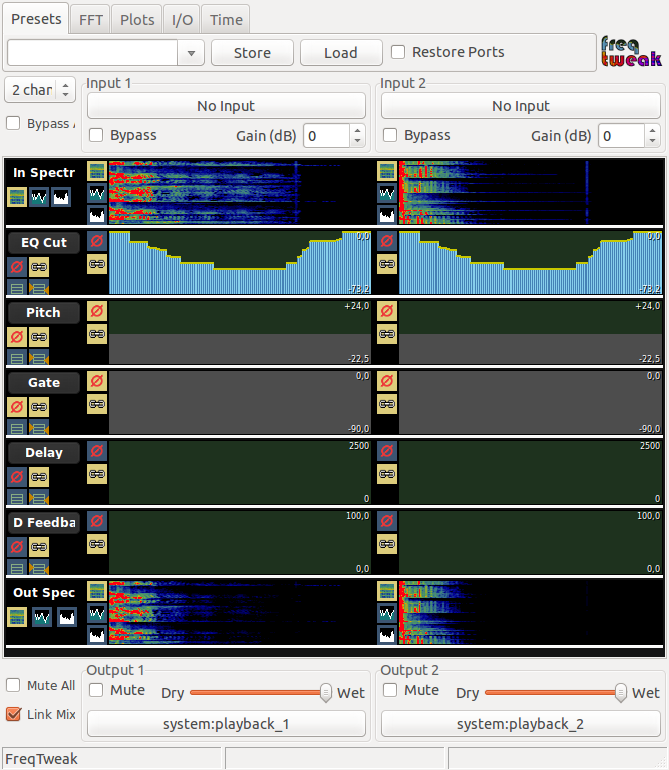
\includegraphics{freqtweak}
\end{center}

% www.free-midi.org

% \begin{comment}
% \section{\href{http://muse-sequencer.org}{MusE}}
% \begin{verbatim}
% $ muse &
% \end{verbatim}
% \begin{center}
%   \includegraphics{muse-connections}  
%   \includegraphics{muse}
% \end{center}
% \end{comment}

\section{\href{http://home.gna.org/fmit}{FMIT (Free Music Instrument Tuner)}}
\begin{verbatim}
fmit &
\end{verbatim}
\begin{center}
  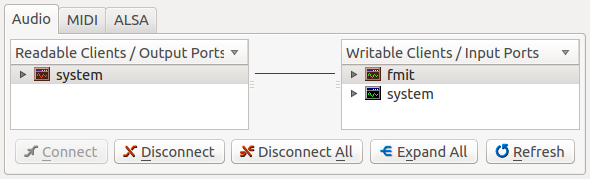
\includegraphics{fmit-connections}  
  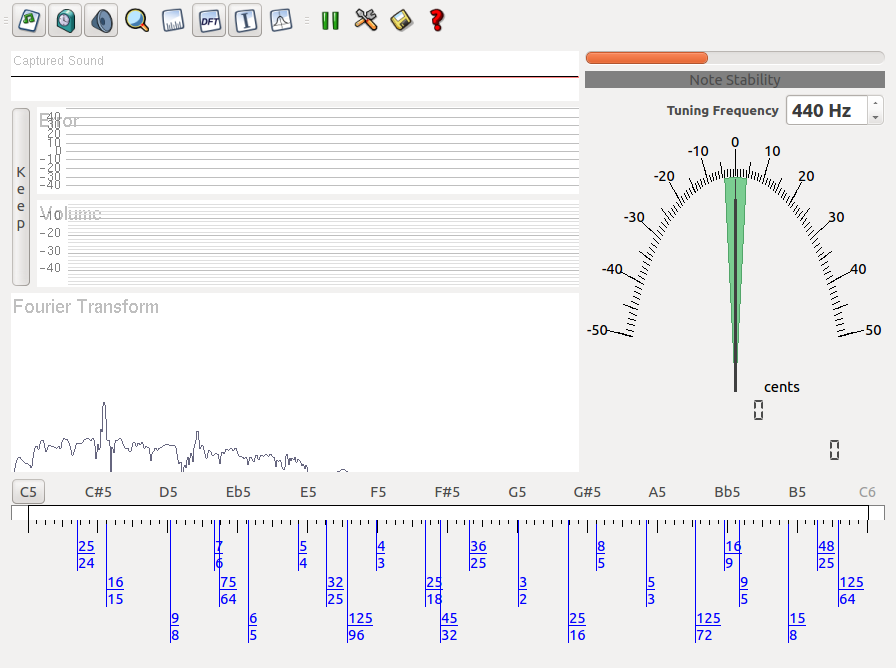
\includegraphics{fmit}
\end{center}

% \begin{comment}
% \section{Rosegarden y MusE: secuenciadores MIDI}
% Un secuenciador como Rosegarden (\url{http://www.rosegardenmusic.com})
% o MusE (\url{http://www.muse-sequencer.org}) son aplicaciones que
% reproducen una secuencia de notas musicales (especificadas normalmente
% usando el sistema MIDI).
% \begin{verbatim}
% sudo apt-get install rosegarden muse
% rosegarden &
% muse &
% \end{verbatim}
% \end{comment}

\chapter{Edition}

\section{\href{http://audacity.sourceforge.net}{Audacity}: capture and edit audio}
%{{{

\begin{verbatim}
# Note: usually audacity establish the connections when playing.
$ audacity &
\end{verbatim}
\begin{center}
  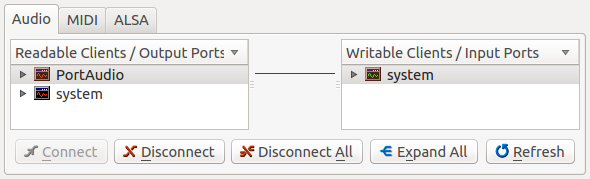
\includegraphics{audacity-connections}
  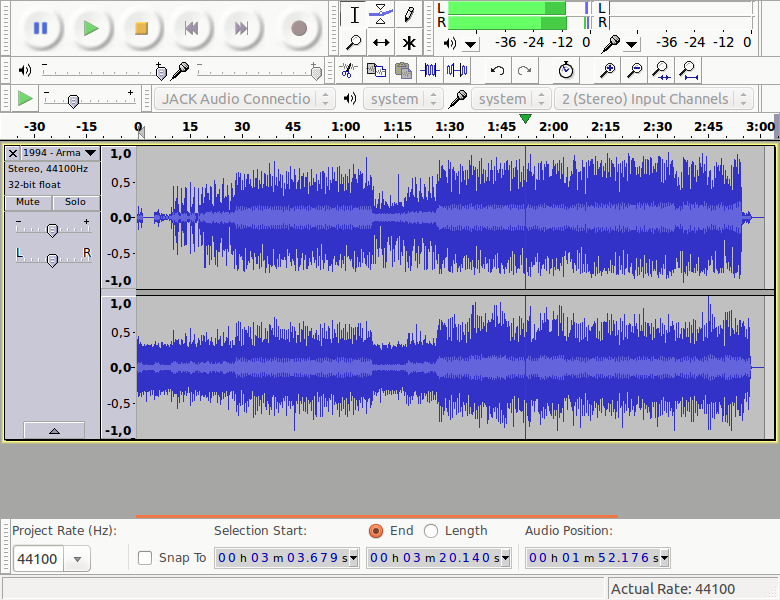
\includegraphics{audacity}
\end{center}

%}}}

\chapter{Capture}

\section{\href{http://plugin.org.uk/timemachine/}{JACK Timemachine}: capture audio}
%{{{

\begin{verbatim}
$ timemachine &
\end{verbatim}
\begin{center}
  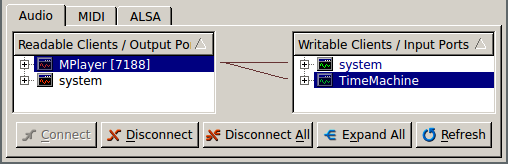
\includegraphics{timemachine-connections}
  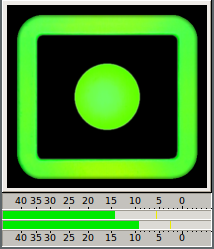
\includegraphics{timemachine}
\end{center}

%}}}

\chapter{Synthesis}

\section{The \href{http://www.hydrogen-music.org/hcms}{Hydrogen} drum machine}
\begin{verbatim}
$ hydrogen &
\end{verbatim}
\begin{center}
  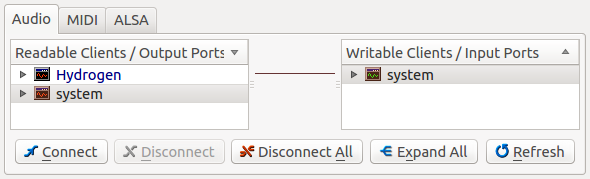
\includegraphics{hydrogen-connections}
  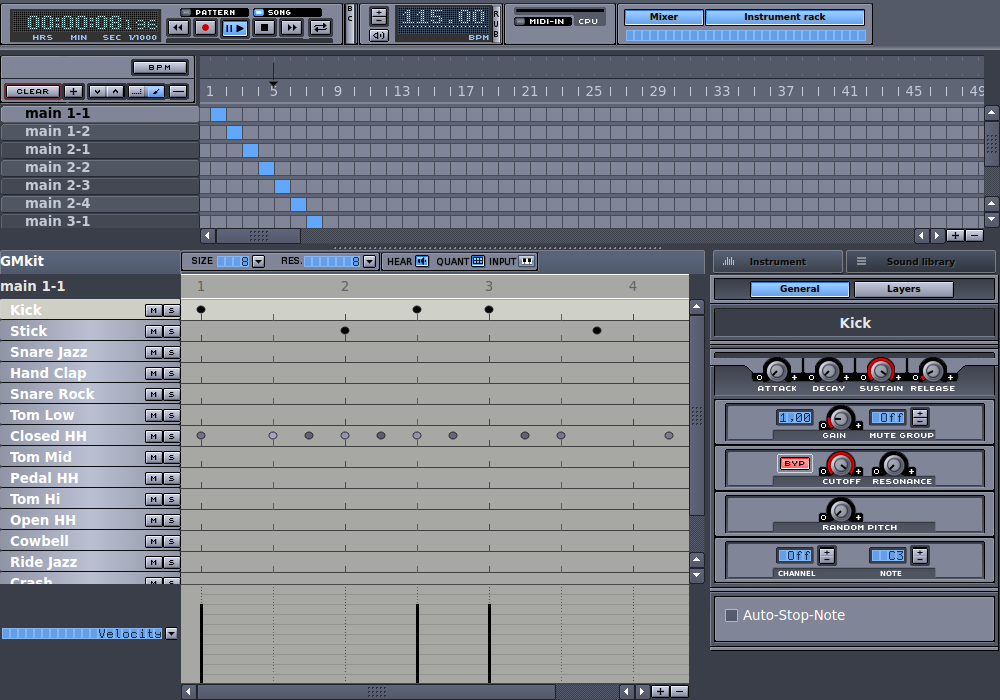
\includegraphics{hydrogen}
  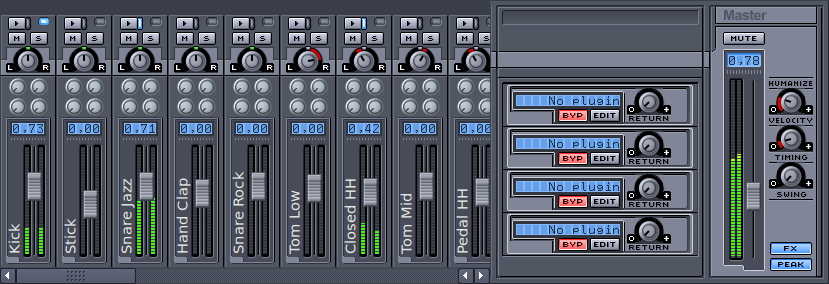
\includegraphics{hydrogen-mixer}
\end{center}

\section{\href{http://zynaddsubfx.sourceforge.net/}{ZynAddSubFX}}
\begin{verbatim}
zynaddsubfx &
\end{verbatim}

\begin{center}
  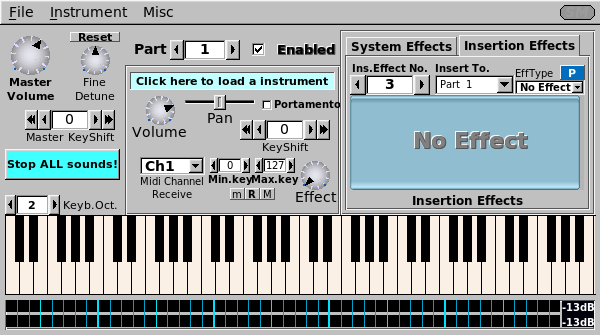
\includegraphics{zynaddsubfx}
  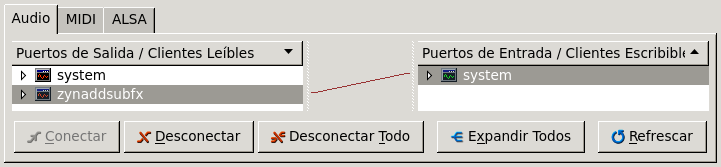
\includegraphics{zynaddsubfx-connections}
\end{center}

\section{\href{http://timidity.sourceforge.net/}{TiMidity}}
\begin{verbatim}
timidity ~/Downloads/teddybear.mid
\end{verbatim}
\begin{center}
  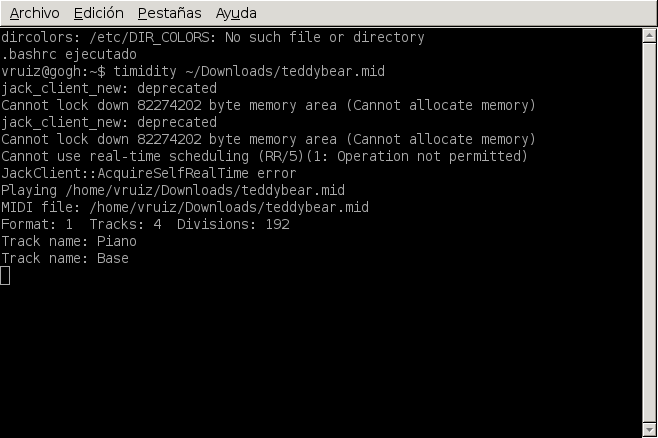
\includegraphics{timidity}
  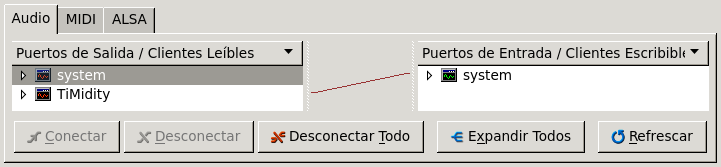
\includegraphics{timidity-connections}
\end{center}

\section{\href{http://jack-keyboard.sourceforge.net/}{JACK Keyboard} and \href{https://code.google.com/p/amsynth/}{AMSynth}}
\begin{verbatim}
jack-keyboard &
amsynth &
\end{verbatim}

\begin{center}
  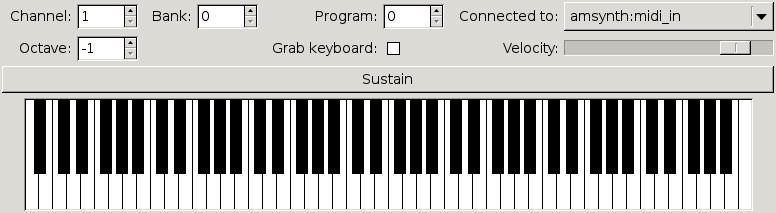
\includegraphics{jack-keyboard}
  %\includegraphics{jack-keyboard-amsynth-connections}
  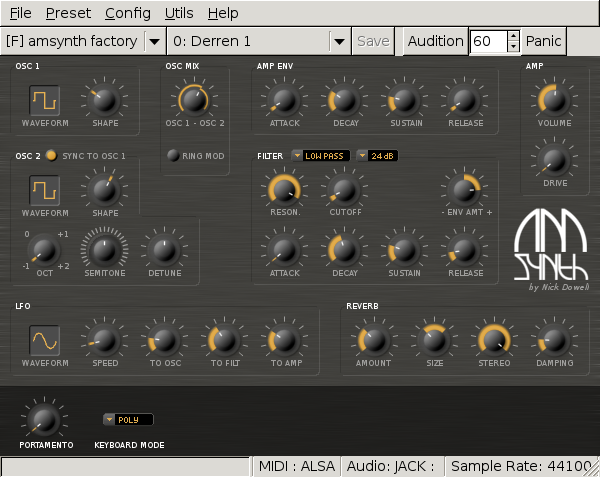
\includegraphics{amsynth}
  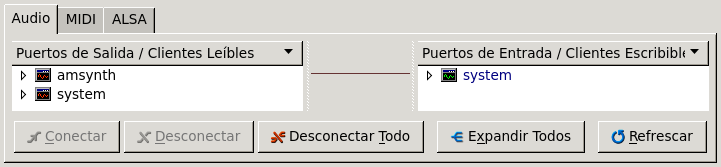
\includegraphics{amsynth-connections}
\end{center}

% \section{PulseAudio sobre JACK}
% JACK es potente pero complejo de usar para aquellos usuarios que no
% son expertos en audio por computadora y por esa raz'on, en la mayor'ia
% de distros de Linux (Ubuntu por ejemplo), el controlador de audio es
% otro diferente, y muchas veces PulseAudio
% (\url{http://www.pulseaudio.org}). Por este motivo, aplicaciones tan
% relevantes como Mozilla Firefox no han sido desarrolladas con soporte
% para JACK.

% Por suerte, los desarrolladores de PulseAudio han desarrollado un
% m'odulo que permite que todas las aplicaciones que usan PulseAudio se
% conecten, desgraciadamente como un todo, a JACK. A pesar de esta
% limitaci'on s'olo visibles desde el punto de vista de JACK, vale la
% pena usar dicho m'odulo porque vamos a poder usar JACK y PulseAudio de
% forma simult'anea.

% La instalaci'on, configuraci'on y uso del m'odulo de PulseAudio para
% JACK se puede realizar como a continuaci'on se especifica:
% \begin{verbatim}
% sudo apt-get install pulseaudio-module-jack
% cd /etc/pulse/
% sudo cp default.pa default.pa.old
% sudo gedit default.pa

% # A~nadir las l'ineas:
% #
% # load-module module-jack-source
% # load-module module-jack-sink
% # al final de la l'inea que posee la cadena: "load-module module-pipe-sink".
% #
% # Por supuesto, estas dos l'ineas NO tienen una "#" al comienzo.
% # Y a continuaci'on comentar todo el bloque (que normalmente se especifica
% # a continuaci'on y que est'a relacionado con "module-udev-detect".

% qjackctl & # Cargamos JACK (si ya no lo est'a).

% # Iniciar JACK (si ya no lo est'a).
% pulseaudio --kill # Reiniciamos PulseAudio

% # Ahora deber'iamos ver los puertos "PulseAudio JACK Sink" y
% # "PulseAudio JACK Source" en la ventaja de conexiones de JACK y
% # conectados como se muestra a continauci'on.
% \end{verbatim}
% \begin{center}
%   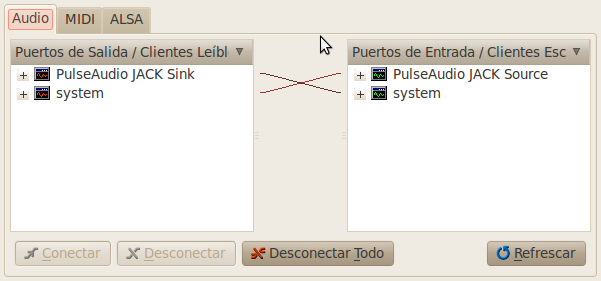
\includegraphics[width=11cm]{PulseAudio-connections}
% \end{center}

\chapter{Remember}
\begin{itemize}

\item While the modules \texttt{module-jack-source} and
  \texttt{module-jack-sink} are loaded into Pulseaudio, the JACK
  server is automatically started.

\item To avoid this, remove these modules from the file
  \texttt{/etc/pulse/default.pa}.

\end{itemize}
